\documentclass[a4paper,12pt,final]{article}

\usepackage[portuges]{babel}
\usepackage[utf8]{inputenc}

\usepackage{fullpage}

\usepackage[T1]{fontenc}
\usepackage[math]{iwona}

\usepackage{amsmath}

\usepackage{graphicx}

\newcommand{\HRule}{\rule{\linewidth}{0.5mm}}

\title{RMEC 13}
\author{Cesar M. Tessarin \and Daniel M. Doine}

\begin{document}

\begin{titlepage}
\begin{center}

\LARGE RMEC 13\\[1cm]

\HRule\\[0.5cm]
{\huge \bfseries Resolução dos Problemas Propostos}
\HRule
\\[8cm]
Cesar M. Tessarin\\
{\large \&}\\
Daniel M. Doine

\vfill

{\large \today}

\end{center}
\end{titlepage}

\section*{Problema 1}
\subsection*{Parte A}
Escrever na forma polar a equação cartesiana $y = x^2$.\\
\\
\underline{Resolução:}\\
\\
Conhecendo `$x = r\cos\theta$' e `$y = r\,\textrm{sen}\,\theta$':
\begin{gather*}
y = x^2\\\\
r\,\textrm{sen}\,\theta = (r\cos\theta)^2\quad\rightarrow\quad
r\,\textrm{sen}\,\theta = r^2\cos^2\theta\quad(\div r)\\\\
\textrm{sen}\,\theta = r\cdot\cos^2\theta\quad(\div \cos\theta)\\\\
r\cdot \cos\theta = \frac{\textrm{sen}\,\theta}{\cos\theta}\quad\rightarrow\quad
r\cdot\cos\theta = \textrm{tg}\,\theta\\\\
\boxed{r = \frac{\textrm{tg}\,\theta}{\cos\theta}}
\end{gather*}

\subsection*{Parte B}
Caracterizar a curva com a equação polar $r = 2\cdot\cos\theta - 4\cdot\,\textrm{sen}\,\theta$.\\
\\
\underline{Resolução:}
\begin{gather*}
\textrm{(Multiplicando a equação por }r\textrm{, e sabendo que }r^2 = x^2 + y^2\textrm{)}\\
r^2 = r(2\cdot\cos\theta - 4\cdot\,\textrm{sen}\,\theta)\quad\rightarrow\quad
r^2 = 2\cdot r\cos\theta - 4\cdot r\,\textrm{sen}\,\theta\quad\rightarrow\quad
\underbrace{x^2 + y^2}_{r^2} = 2x - 4y\\
\textrm{(Completando os quadrados perfeitos)}\\
x^2 - 2x + y^2 + 4y = 0\quad\rightarrow\quad x^2 - 2x + 1 + y^2 + 4y + 4 = 1 + 4\\\\
\boxed{(x - 1)^2 + (y + 2)^2 = 5}\\
\boxed{\textrm{Uma circunferência com o centro em }(1,-2)\textrm{ e raio }\sqrt{5}}\\\\
\textit{Fórmula geral de uma circunferência de centro }(a,b)\textrm{ e raio }r\textrm{:}\\
\boxed{(x - a)^2 + (y - b)^2 = r^2}
\end{gather*}
\newpage

\section*{Problema 2}

O primeiro passo a ser tomado é encontrar a coordenada de cada ponto. Sem seguir a ordem alfabética, temos:

\subsection*{Ponto E}
Nota-se que está a mesma ``altura'' do ponto da parábola que cruza o eixo \emph{y}. Logo, $y_E = 12$ \textit{(Função: $y = x^2 - 6x + \textbf{\underline{12}}$)}.\\
Aplicando $y_E$ na função obtemos seu $x$:\\
\begin{gather*}
12 = x^2 - 6x + 12\quad\rightarrow\quad
x^2 - 6x = 0\quad\rightarrow\quad
x(x - 6) = 0\\\\
\left\{\begin{array}{rl}
x' \rightarrow 0 & (\textrm{Intersecção com eixo }y)\\
x'' \rightarrow 6 &
\end{array}\right.
\end{gather*}

$$\boxed{E(6,12)}$$

\subsection*{Ponto D}
Simplesmente observando o gráfico:
\boxed{D(20,0)}

\subsection*{Ponto C}
Obviamente: \boxed{C(0,0)}

\subsection*{Ponto B}
A reta mostrada intercepta a parábola em dois pontos ($B$ e $E$). Sabemos ainda que (-10,0) pertence a esta reta. Assim, podemos calcular sua função:
\begin{gather*}
m = \frac{\Delta y}{\Delta x}\quad\rightarrow\quad
m = \frac{12 - 0}{6 - (-10)}\quad\rightarrow\quad
m = \frac{12}{16} = \boxed{\frac{3}{4}}\\\\
(y - y_0) = m(x - x_0)\quad\rightarrow\quad
(y - 0) = \frac{3}{4}(x + 10)\quad\rightarrow\quad
\boxed{y = \frac{3}{4}x + \frac{15}{2}}\\
\\
\frac{3}{4}x + \frac{15}{2} = x^2 - 6x + 12\quad(\times 4)\quad\rightarrow\quad
3x + 30 = 4x^2 - 24x + 48\quad\rightarrow\quad
\boxed{4x^2 - 27x +18 = 0}\\
\end{gather*}

\newpage

\begin{gather*}
\Delta = b^2 - 4ac\quad\rightarrow\quad
\Delta = 27^2 - 4\cdot 4\cdot 18\quad\rightarrow\quad
\Delta = 729 - 288\quad\rightarrow\quad
\Delta = 441\\\\
x' = \frac{-b + \sqrt{\Delta}}{2a}\quad\rightarrow\quad
x' = \frac{27 + 21}{8}\quad\rightarrow\quad
\boxed{x' = 6}\\
x'' = \frac{-b + \sqrt{\Delta}}{2a}\quad\rightarrow\quad
x'' = \frac{27 - 21}{8}\quad\rightarrow\quad
\boxed{x'' = \frac{3}{4}}
\end{gather*}
$x'$ já era um ponto conhecido. Assim, $x_B = x''$. Para calcular seu $y$:
\begin{gather*}
y_B = \frac{3}{4}x + \frac{15}{2}\quad\rightarrow\quad
y_B = \frac{3}{4}\cdot\frac{3}{4} + \frac{15}{2}\quad\rightarrow\quad
y_B = \frac{9}{16} + \frac{15}{2}\quad\rightarrow\quad
\boxed{y_B = \frac{129}{16}}\\
\boxed{B\left(\frac{3}{4},\frac{129}{16}\right)}
\end{gather*}

\subsection*{Ponto A}
Vértice da função. Pode ter seu $x$ descoberto facilmente pela média de pontos simétricos, como E e o ponto de intersecção com o eixo $y$:
\begin{gather*}
\frac{6 + 0}{2} = 3\,,\quad\longrightarrow\quad
y_A = x_A^2 - 6x_A + 12\quad\rightarrow\quad
y_A = 3^2 - 6\cdot 3 + 12\quad\rightarrow\quad
y_A = 3\\\\
\boxed{A(3,3)}
\end{gather*}

\subsection*{Calculando a área}
Através da fórmula demonstrada por F.P.Garpelli, temos:
\begin{gather*}
S = \frac{1}{2}\times
\left\langle\begin{array}{ccccc}
x_A & x_B & x_C & x_D & x_E\\
y_A & y_B & y_C & y_D & y_E
\end{array}\right\rangle\quad\rightarrow\quad
S = \frac{1}{2}\times
\left\{\begin{array}{cccccc}
x_A & x_B & x_C & x_D & x_E & x_A\\
y_A & y_B & y_C & y_D & y_E & y_A
\end{array}\right\}\\\\
S = \frac{1}{2}\times
\left\{\begin{array}{cccccc}
3 & \frac{3}{4} & 0 & 20 & 6 & 3\\[.1cm]
3 & \frac{129}{16} & 0 & 0 & 12 & 3
\end{array}\right\}\\\\
S = \frac{1}{2}\times\left\{\left(3\cdot \frac{129}{16} + 0 + 0 + 240 + 18\right) - \left(3\cdot\frac{3}{4} + 0 + 0 + 0 + 36\right)\right\}\\\\
S = \frac{1}{2}\times\left\{\frac{387}{16} + 258 - \frac{9}{4} - 36\right\}\quad\rightarrow\quad
S = \frac{1}{2}\times\left\{222 + \frac{351}{16}\right\}\quad\rightarrow\quad
S = 111 + \frac{351}{32}
\end{gather*}\\
Como $352 \div 32 = 11$, pode-se dizer que $\boxed{S \approx 122}$

\newpage

\section*{Problema 3}

O primeiro passo, é posicionar a base e construir sobre ela um triângulo com os dois lados não paralelos:\\\\
\begin{center}
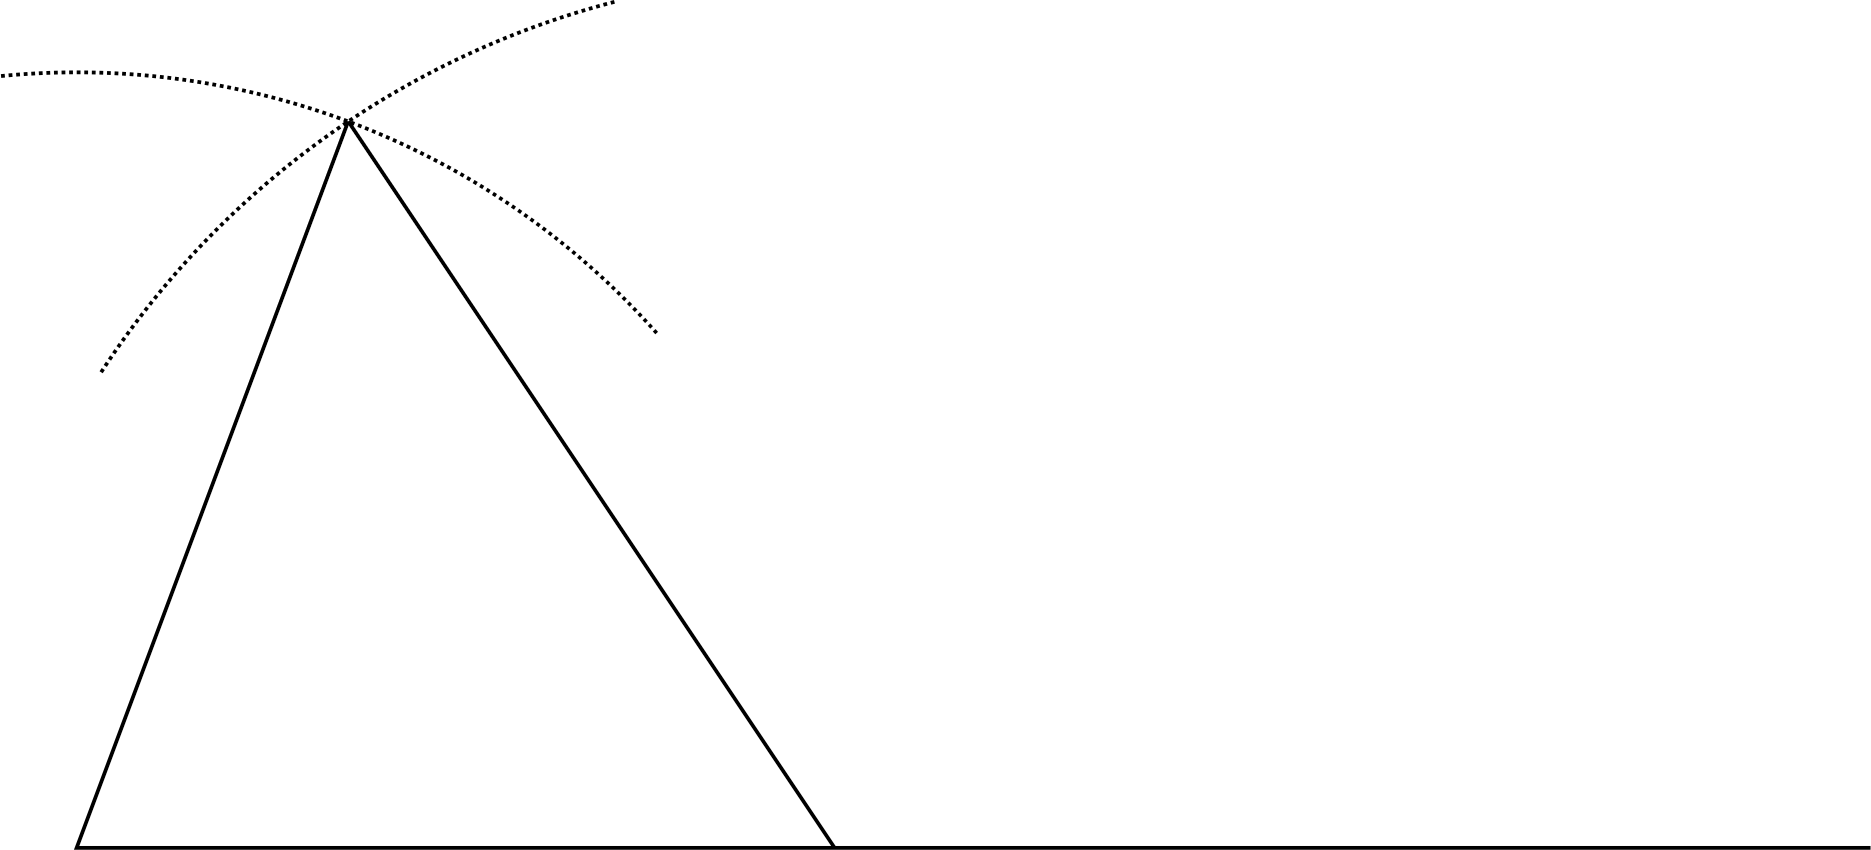
\includegraphics[scale=.12]{passo1}
\end{center}
\vfill
Em seguida, basta deslocar um dos lados para a outra extremidade da base e adicionar o 4$^{\circ}$ lado (paralelo com a base):\\\\
\begin{center}
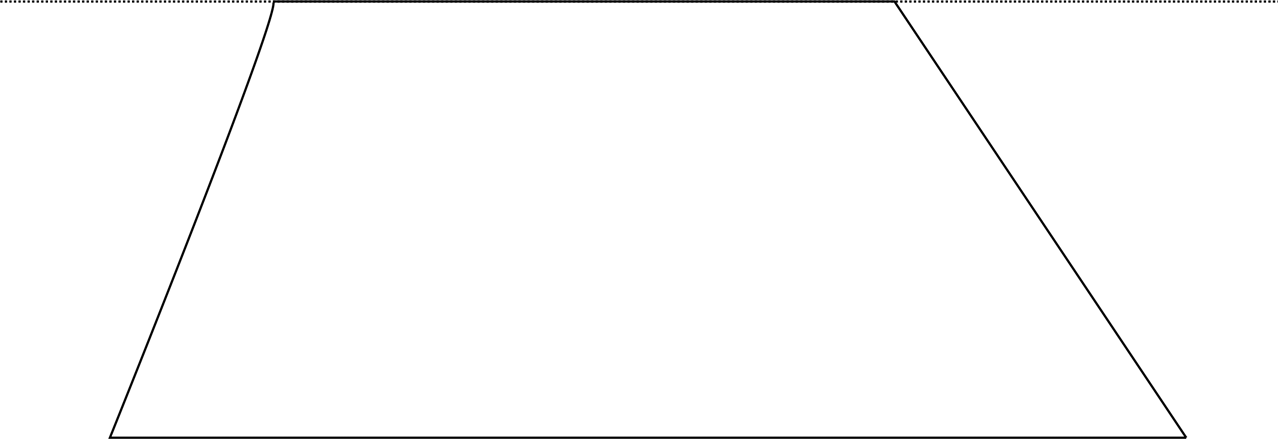
\includegraphics[scale=.18]{passo2}
\end{center}
\vfill
Formando o trapézio:
\vfill
\begin{center}
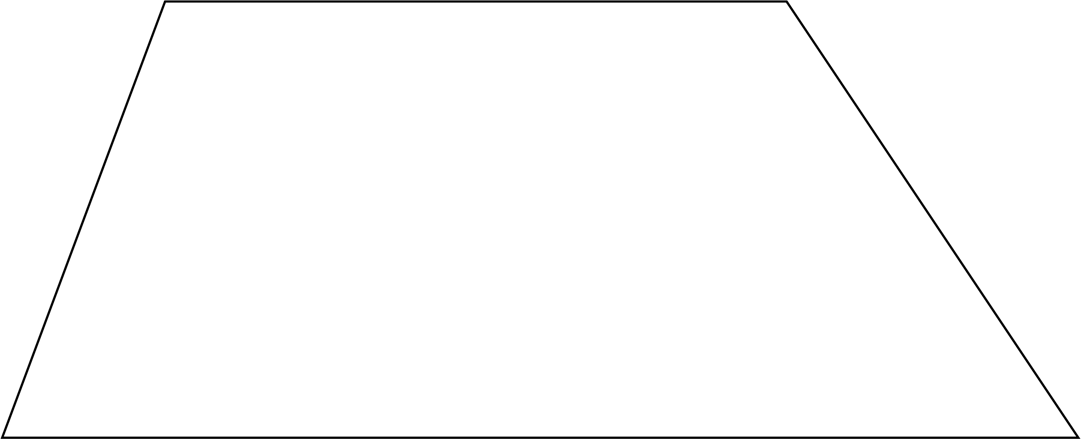
\includegraphics[scale=.25]{passo3}
\end{center}
\vfill

\end{document}